%\documentclass[11pt,a4paper]{report}
\documentclass{article}
\usepackage[top=1in, bottom=1in, left=1in, right=1in]{geometry}

%%%%%%%%%%%%%%%%
%%% PACKAGES %%%
%%%%%%%%%%%%%%%%

\usepackage{amsmath,amssymb}
\usepackage{graphicx}
\usepackage{parskip}

% used with figures:
\usepackage{float}
\usepackage{caption}
\usepackage{subcaption}

\graphicspath{{./img/}}

\usepackage[toc,page,title,titletoc]{appendix}

\title{computer gestuurde regeltechnieken - Part 2}
\author{Willem Melis (r0348639)}
\date{\today}

\setcounter{MaxMatrixCols}{20}


\begin{document}

\begin{titlepage}
\begin{center}


\includegraphics[width=3cm]{kuleuven.jpg}~\\[1cm]
\vfill


\textsc{\LARGE KU Leuven}\\[0.7cm]

\textsc{\Large Computer gestuurde regeltechnieken}\\[0.7cm]
\textsc{\Large Exercises - Part 1 }\\[0.7cm]



\centering \huge \bfseries Case study: Quadcopter

\end{center}

\vfill

% auteurs et tuteur
\begin{center}
\emph{Author:} \\[.2cm]
\begin{tabular}[h]{rl}
Willem \textsc{Melis} & r0348639\\
\phantom{------------------------} & \phantom{------------------------}\\
\end{tabular}
\end{center}

\vfill

\begin{center}
\begin{tabular}[h]{rl}
\emph{Professor:} & Bart \textsc{De Moor} \\
\emph{Assistants:}&  
Oscar Mauricio  \textsc{Agudelo} \\
&  Supinya  \textsc{Piampongsant} \\
\phantom{------------------------} & \phantom{------------------------}\\
\end{tabular}
\end{center}

\vfill
\vfill
\vfill

%date
\begin{center} 
2016 - 2017 \\[.5cm]
{\Large \today}
\end{center}

\end{titlepage}

\tableofcontents 
\newpage

\section{Introduction}
The report tries to follow the order of the assignment as much as possible. For each part there is Matlab code, the appendix briefly explains which files belong to which part of the report. Some of the figures are added as an appendix. The text specifically refers to them when the reader should take a look at them, they are of little value on there own.
\section{The cost function}
\subsection{Formulation}
The coordinates of the end of the two arms are $p_1$ and $p_2$ are easily determined with simple geometric formula\'s. 
$$\triangle x=cos(\theta) \cdot d$$
$$\triangle y = sin(\theta) \cdot d$$
$$p_1=(x_{k}+\triangle x,y_{k}+\triangle y) = (x_{p_1},y_{p_1})$$
$$p_2=(x_{k}-\triangle x,y_{k}-\triangle y) =  (x_{p_2},y_{p_2})$$

The points $p_1$ and $p_2$ can then be used to determine the area covered by the goalkeeper. A straight line starting from the attackers position and going trough one of these points will hit the x-axis at the borders of the area. 

The rico of the line using the first point $p_1$ and the attackers position is $a = \frac{y_{a}-y_{p_1}}{x_{a}-x_{p_1}}$ . The function describing the line then becomes equation equation~\ref{eq:simple function describing line trough p1}
\begin{equation}
	f(x) = a (x-x_{p_1}) + y_{p_1}
	\label{eq:simple function describing line trough p1}
\end{equation}

Some simple algebra will show that $f(x)=0$ occurs if $x=x_{p_1}-a^{-1}\cdot y_{p_1}$. These points are visible on figure~\ref{eq:simple function describing line trough p1} with the green line crossing the x-axis. The smallest of the two x values is the left side and the largest the right side. Now the only thing left is to take the difference with the border of the goal.

Nothing was mentioned in the assignment about what should happen if the area covered by the goalkeeper is outside the goal area. So if the cost function should reward or punish a goalkeeper that covers more then just the goal. In this report its assumed that the goalkeeper should try to cover only the goal. Nothing more or less then that. Thats why absolute value of the difference is saved, everything that is covered outside the goal area adds up to the cost function.  $xl=|zl+goalWidth/2|$ and $xr=|goalWidth/2-zr|$ with zl and zr the coordinates of the 2 borders of the area covered by the goalkeeper.

This means that the cost function of $x_l$ and $x_r$ is semi-positive definite. Which is an excellent properties to have when working with optimization algorithms.Later on $x_l$ and $x_r$ will be squared and added up which would make it semi-positive definite anyway

Although the assignment did not require this it seems safer to make sure that the cost function has no optima outside the allowed goalkeeper area. When the goalkeeper moves out of the penalty area the closest coordinates inside the area are used instead. The cost function then adds the difference from the border value as penalty to the cost value. The penalty is added because derivative driven optimization algorithms don't like flat areas at all. And this ensures that no local minimum can be found outside the penalty area. As at least 1 border value is lower. It might be clever to put the difference between the unfeasible point and the closest border coordinates to a high power. To make the unfeasible area very steep and move gradient based algorithms away from it.


\begin{figure}[H]
	\centering
	\includegraphics[width=0.5\textwidth]{./costFunction/simpleDemo.png}
	\caption{simple demo using $x_a = 10$,$y_a=17$ from table 1 in the assignment and goalkeeper with $\theta=\frac{\pi}{1.3}$ x=1 and y=3. The blue line describes the arms, the red line is a straight line between the attack and the goal keeper. And finally the green lines describe the area covered by the goalkeeper}
	\label{fig:simple demo}
\end{figure}

\subsection{Optimizing the cost function}

The cost function is defined as $J=x_r^2+x_l^2$  figure~\ref{fig:simple demo J}. The resulting graph of J with a fixed $\theta$ seems to indicate that this cost function is convex if the goalkeeper stays inside the penalty area and $|\theta| \leq \pi $. And the attacker is at the position given in the assignment.

However if the goalkeeper can move out of the penalty area or if the attacker can go inside the penalty area things change drastically. Local optima will start to appear, and the problem is certainly not convex any more.

The Cost function is periodic in function of $\theta$ as $\theta$ is not limited between for example $- \pi$ and $+ \pi$. This can be remedied by adding an constraint in the optimization or adding an additional penalty as was done when moving outside the penalty area.

So if $theta$ is fixed then the function is convex except for the penalty area borders that are very sharp (left and right derivative is not equal, very dangerous). If a smoothing technique would be applied then this could become convex.(if $\theta$ is fixed)

Figure~\ref{fig:simple demo J} contains the value of the log of the cost function solely in function of x $\theta$ and y are constant. There appears to be a nice global optimum. Figure~\ref{fig:simple demo J surf} contains a 3D plot of log the cost function with $\theta=0$, $x \in [-30,30]$ and $y \in [-10,50]$.

\begin{figure}[H]
	\centering
	\includegraphics[width=0.5\textwidth]{./costFunction/simpleDemoJ.png}
	\caption{ attacker: $x_a = 10$,$y_a=17$ goalkeeper: $\theta=0$ $y \in[-10,10]$ and y=3 the top plot contains $x_l$ and $x_r$ separate while the bottom plot contains J ($J=x_r^2+x_l^2$)}
	\label{fig:simple demo J}
\end{figure}

\begin{figure}[H]
	\centering
	\includegraphics[width=0.5\textwidth]{./costFunction/simpleDemoJSurf.png}
	\caption{simple demo using $x_a = 10$,$y_a=17$ from table 1 in the assignment and goalkeeper with $\theta=0$ $x \in [-30,30]$ and  $y \in [-10,50]$ $J=x_r^2+x_l^2$}
	\label{fig:simple demo J surf}
\end{figure}

Remark: Figure~\ref{fig:simple demo J surf} and figure~\ref{fig:simple demo J} only seem to be flat outside the penalty area, as the small difference is not visible on the log scale.

\subsection{Formulate the optimization problem}
Because the cost function by definition cannot have an optimal point outside the goalkeeper it is not mandatory to include these conditions. However the border of the goalkeeper area has an dangerous corner on the cost function. It seems safer to include the goalkeeper area and it can't hurt to give the optimizer more information. $\theta$ is chose to be between 0 and $\pi$. 
\begin{equation}
	\begin{aligned}
	& \min_{x,y,\theta}
	& & costFunction(x,y,\theta)\\
	& \text{subject to}
	& & 0 \leq y \leq y_{max}\\
	&&& |x| \leq x_{max} \\
	&&& -\pi \leq \theta \leq \pi \\
	\end{aligned}
	\label{eq:goalkeeper optimization formulation}
\end{equation}
\section{Dynamic keeper model}
\subsection{Statespace model}
\begin{equation}
\begin{cases}
	\dot{x} = v_x \\
	\dot{y} = v_y \\
	\dot{\theta}=\omega \\
	\dot{v_x} = \frac{1}{m}(F_x - \rho v_x)\\
	\dot{v_y} = \frac{1}{m}(F_y - \rho v_y)\\
	\dot{v_z} = \frac{1}{I}(M - 0.01\omega)\\
\end{cases}
\label{eq:basic model keeper}
\end{equation}

Equation \ref{eq:basic model keeper} can be converted into a state space model(equation~\ref{eq:full statepace model goalkeeper}) of the form: $\dot{x} = Ax+Bu$  with $x=[x y \omega v_x v_y v_z]$ and $u=[F_x F_y M]$

\begin{equation}
\begin{bmatrix}
\dot{x} \\
\dot{y} \\
\dot{\omega} \\
\dot{v_x} \\
\dot{v_y} \\
\dot{\omega} \\
\end{bmatrix}
=
\begin{bmatrix}
0 & 0 & 0 & 1 & 0 & 0 \\
0 & 0 & 0 & 0 & 1 & 0 \\
0 & 0 & 0 & 0 & 0 & 1 \\
0 & 0 & 0 & \frac{-\rho v_x}{m} & 0 & 0 \\
0 & 0 & 0 & 0 &\frac{-\rho v_y}{m} & 0 \\
0 & 0 & 0 & 0 & 0 & -0.01 \\
\end{bmatrix}
\begin{bmatrix}
x \\
y \\
\omega \\
v_x \\
v_y \\
\omega \\
\end{bmatrix}
+
\begin{bmatrix}
0 & 0 & 0 \\
0 & 0 & 0 \\
0 & 0 & 0 \\
m^{-1} & 0 & 0 \\
0 & m^{-1} & 0 \\
0 & 0 & I^{-1} \\
\end{bmatrix}
\begin{bmatrix}
F_x \\
F_y \\
M \\
\end{bmatrix}
\label{eq:full statepace model goalkeeper}
\end{equation}

\subsection{Discrete-time state space model: Eulers rule}

\subsubsection{Symbolic expressions discrete matrices}
\begin{equation}
	\begin{cases}
		Ad = eye(6) + Ts*A \\
		Bd = Ts*B \\
		Cd = C \\
		Dd = D \\
	\end{cases}
\end{equation}

$$
A_d=
\begin{bmatrix}
1 & 0 & 0 & T_s & 0 & 0 \\
0 & 1 & 0 & 0 & T_s & 0 \\
0 & 0 & 1 & 0 & 0 & T_s \\
0 & 0 & 0 & 1 - \frac{\rho v_x}{m}T_s & 0 & 0 \\
0 & 0 & 0 & 0 & 1 - \frac{\rho v_7}{m}T_s & 0  \\
0 & 0 & 0 & 0 & 0 & 1-0.01T_s \\
\end{bmatrix}
$$
$$
B_d=
\begin{bmatrix}
0 & 0 & 0 \\
0 & 0 & 0 \\
0 & 0 & 0 \\
m^-1T_s & 0 & 0 \\
0 & m^-1T_s & 0 \\
0 & 0 & I^{-1}T_s \\
\end{bmatrix}
\ 
C_d=
\begin{bmatrix}
1 & 0 & 0 & 0 & 0 & 0 \\
0 & 1 & 0 & 0 & 0 & 0 \\
0 & 0 & 1 & 0 & 0 & 0 \\
\end{bmatrix}\ 
D_d=
\begin{bmatrix}
0 & 0 & 0 \\
0 & 0 & 0 \\
0 & 0 & 0 \\
\end{bmatrix}
$$

\subsubsection{Numerical values discrete matrices}
$$
A_d=
\begin{bmatrix}
	1 & 0 & 0 & 0.15 & 0 & 0 \\
	0 & 1 & 0 & 0 & 0.15 & 0 \\
	0 & 0 & 1 & 0 & 0 & 0.15 \\
	0 & 0 & 0 & 0.9667 & 0 & 0 \\
	0 & 0 & 0 & 0& 0.9667 & 0  \\
	0 & 0 & 0 & 0 & 0 & 0.9992 \\
\end{bmatrix}
$$
$$
B_d=
\begin{bmatrix}
0 & 0 & 0 \\
0 & 0 & 0 \\
0 & 0 & 0 \\
0.0017 & 0 & 0 \\
0 & 0.0017 & 0 \\
0 & 0 & 0.0833 \\
\end{bmatrix}
\ 
C_d=
\begin{bmatrix}
1 & 0 & 0 & 0 & 0 & 0 \\
0 & 1 & 0 & 0 & 0 & 0 \\
0 & 0 & 1 & 0 & 0 & 0 \\
\end{bmatrix}
\ 
D_d=
\begin{bmatrix}
0 & 0 & 0 \\
0 & 0 & 0 \\
0 & 0 & 0 \\
\end{bmatrix}
$$

\subsubsection{Analysis}
Figure~\ref{fig:zplot euler} contains a plot of the z domain with the poles and transmission zeros. The poles are all within the unit circle, so the system is stable. Its is important to check this as the Euler rule does not guarantee a stable discrete system if the continuous system is stable. There are no transmission zeros.

The rank of the controllability matrix is 6 with the lowest singular value being 0.00099, the system is observable. The rank of the observability matrix is 6 with the lowest singular value being 0.55, the system is observable.

As the system is stable  the system is stabilisable. And as the system is observable, the system is detectable.

The system is minimum.


\begin{figure}[H]
	\centering
	\includegraphics[width=0.3\textwidth]{./keeperModel/zplotEuler.eps}
	\caption{zplot of the discrete system system with Euler's rule}
	\label{fig:zplot euler}
\end{figure}

\subsection{Discrete-time state space model: bilinear transformation}
Figure~\ref{fig:zplot bil} contains a plot of the z domain with the poles and transmission zeros. The poles are all within the unit circle, so the system is stable. The bilinear  transformation always maps all stable poles from the continuous system to stable poles of the discrete system. All 6 of the transmission zeros are within the unit circle at -1 This means the the system is a minimum phase system.

The bilinear transformation always maps the stable poles/zeros from the continuous system over the whole unit circle. This makes the bilinear transformation the most elegant of the 4 methods tried in this report. And so the preferred method if the other methods have similar properties.

The rank of the controllability matrix is 6 with the lowest singular value being 0.00095, the system is observable. The rank of the observability matrix is 6 with the lowest singular value being 0.52, the system is observable.

As the system is stable  the system is stabilisable. And as the system is observable, the system is detectable.

The system is minimum.

\begin{figure}[H]
	\centering
	\includegraphics[width=0.3\textwidth]{./keeperModel/zplotBil.eps}
	\caption{zplot of the discrete system system with the bilinear transformation}
	\label{fig:zplot bil}
\end{figure}

\subsection{Discrete-time state space model: zero order hold}
Figure~\ref{fig:zplot zoh} contains a plot of the z domain with the poles and transmission zeros. The poles are all within the unit circle, so the system is stable. All 3 of the transmission zeros are within the unit circle at about -1 This means the the system is a minimum phase system.

The rank of the controllability matrix is 6 with the lowest singular value being 0.0009, the system is observable. The rank of the observability matrix is 6 with the lowest singular value being 0.54, the system is observable.

As the system is stable  the system is stabilisable. And as the system is observable, the system is detectable.

The most significant property of the zero and hold method is that it is a step invariant method. Which means that its step impulse is the same as that of the continuous system. This properties is discussed later on in this section when the step impulses are discussed.

The system is minimum.

\begin{figure}[H]
	\centering
	\includegraphics[width=0.3\textwidth]{./keeperModel/zplotZOH.eps}
	\caption{zplot of the discrete system system with zero order hold}
	\label{fig:zplot zoh}
\end{figure}

\subsection{Discrete-time state space model: backward rectangle}
Figure~\ref{fig:zplot backr} contains a plot of the z domain with the poles and transmission zeros. The poles are all within the unit circle, so the system is stable. All 6 of the transmission zeros are within the unit circle at about 0, some positive some negative. This means the the system is not a minimum phase system. Numerical errors of size $10^-6$ are a lot higher then  $10^{-15}$( machine precision).

The backward rectangle method can only map the stable continuous poles onto stable discrete poles in the circle between 0 and 1. This means that not the entire unit circle is used, in contrast to the bilinear transformation.

The rank of the controllability matrix is 6 with the lowest singular value being 0.0009, the system is observable. The rank of the observability matrix is 6 with the lowest singular value being 0.5, the system is observable.

As the system is stable  the system is stabilisable. And as the system is observable, the system is detectable.

The system is minimum.

\begin{figure}[H]
	\centering
	\includegraphics[width=0.3\textwidth]{./keeperModel/zplotbackr.eps}
	\caption{zplot of the discrete system system with backward rectangle}
	\label{fig:zplot backr}
\end{figure}

\subsection{Step responses}
Figure~\ref{fig:step responese disc}(in the appendix) contains all the full impulse responses for the first 4 seconds. A step impulse on $F_x$ obviously has little influence on $y$ or $\theta$. Same goes for $F_y$ or $M$, only the diagonal elements are useful. Figure~\ref{fig:step response diag} contains the 3 relevant plots for a step impulse with a simulation time of 2 seconds. 

As mentioned before the zero order hold method is step invariant and so obviously has the best results. The bilinear and forward euler are about equally good and the backward rectangle has the worst step response of all.

\begin{figure}[H]
	\centering
	\begin{subfigure}[b]{0.45\textwidth}
		\includegraphics[width=\textwidth]{./keeperModel/step_impulse_total_1.png}
		\caption{step response on $F_x$}
	\end{subfigure}
	\begin{subfigure}[b]{0.45\textwidth}
		\includegraphics[width=\textwidth]{./keeperModel/step_impulse_total_2.png}
		\caption{step response on $F_y$}
	\end{subfigure}
	\begin{subfigure}[b]{0.45\textwidth}
		\includegraphics[width=\textwidth]{./keeperModel/step_impulse_total_3.png}
		\caption{step response on $M$}
	\end{subfigure}
	\caption{step impulse on different imputs}
	\label{fig:step response diag}
\end{figure}

\subsection{Selection of transformation method}
Without looking at any of the results the bilinear transformation seems to be the most obvious option. As it maps over the entire unit circle and is always stable if the continuous system was stable. This was confirmed by the numerical experiments. The transfer-function will change less drastically if the poles and zeros are further away, this will have an effect on the smoothness of the reference inputs. 

When in a later stage the transformation is used to determine the set points, its very noticeable that the reference inputs are the smoothest with the bilinear transformation. And so the bilinear transformation was chose as the discrete transformation method.
\section{Setpoint}

\subsection{A first approach}

The theoretical trajectory is displayed in figure~\ref{fig:trajectory}. The coordinates of the trajectory are obviously the x and y state of the keeper. The remaining question is: what are the appropriate inputs to reach these states? Notice that the trajectory starts from (0,0) which slightly simplifies the formula's.

\begin{figure}[H]
	\centering
	\includegraphics[width=0.5\textwidth]{./setpoint/traject.png}
	\caption{The theoretical trajectory}
	\label{fig:trajectory}
\end{figure}

A simple approach is to minimize $J_N = \sum_{k=0}^{N-1} (w_k-y_k)^T(w_k-y_k)$. This is realized with the formula on top of page 127 $u_{opt}=(\mathcal{H}_N^T\mathcal{H}_N)^{-1}\mathcal{H}_N^T(w-\mathcal{O}_nx_0)$, in which $x_0$ can be left out as its zero. The final equation then becomes equation~\ref{eq:least squares optimalisation formula}. After the $u_{ref}$ values are determined for the $x_{ref}$, $u_{ref}$ is used to simulate the system. 

\begin{equation}
u_{opt}=(\mathcal{H}_N^T\mathcal{H}_N)^{-1}\mathcal{H}_N^Tw
\label{eq:least squares optimalisation formula}
\end{equation}

Figure~\ref{fig:least square opti simulation} contains the output of the simulation. The top of figure~\ref{fig:least square opti simulation}  contains the actual trajectory and the bottom contains the $u_{ref}$ used for that trajectory. At first sight this might seem perfect as the goalkeeper perfectly follows the trajectory. However the $u_{ref}$ tells a who different story, $u_{ref}$ is oscillating a lot between extremely high values. $F_{max}$ is of size $10^2$ while $u_{ref}$ contains an $F_x$ of size $10^6$.

Besides the bad $u_ref$ there is an other problem. The matrix $\mathcal{H}_N^T\mathcal{H}_N$ has a condition number of about $10^{21}$. The machine precision that was used is $10^{-15}$, this means the calculations are correct for zero digits. 

\begin{equation}
u_{opt}=(R+\mathcal{H}_N^TQ\mathcal{H}_N)^{-1}\mathcal{H}_N^TQw
\label{eq:least squares optimalisation formula with R and Q}
\end{equation}

\subsection{Lowering the condition number}

An simple way to increase the condition number of a matrix is to add a unit matrix. And so make all the columns of the matrix $\mathcal{H}_N^T\mathcal{H}_N$ more orthogonal to each other. The course notes on page 131 do exactly this. (and more)
Instead of optimizing  $J_N = (w-y)^T(w-y)$ 2 extra weight matrices $Q$ and $R$ are added : $J_N = u^TRu + (y-w)^TQ(y-w)$. ($u_opt$ now becomes equation~\ref{eq:least squares optimalisation formula with R and Q}) Q is taken as a unit matrix and R is taken as a diagonal matrix with $10^{-4}$ on its diagonal. This will reduce the condition from $10^{21}$ to  $10^{9}$. Now we have 6 significant digits of  accuracy (not taking in account numerical errors as they will be small ). At first one may think that 6 significant digits is not a lot to work with, but consider the fact that there's no guarantee the model itself is correct at 6 digits.

When using a regularization diagonal matrix with $10^{-4}$ the LQR will give very good results. And the MPC will give similar results. Because the LQR has such a good results it leaves no room for the MPC improve the situation. This is why a regularization parameter of $10^{-5}$ was chosen instead of the nice $10^{-4}$. The LQR will have trouble taking the last corner, however the MPC with a horizon of 2N will be able to take that corner very well. And the final result for the MPC with horizon 2N will be better with $10^{-5}$ then  $10^{-4}$.

In short, if only the LQR was used, then $10^{-4}$ is the better option. However the MPC has better results with $10^{-5}$ .

\subsection{Final results}

The results of these new $u_ref$ values is displayed in figure~\ref{fig:least square opti simulation, better condition}. The trajectory is not as good as with the bad conditioned matrix but the $u_ref$ now contains reasonable values. This is actually useful for the application itself.

\begin{figure}[H]
	\centering
	\begin{subfigure}[b]{0.45\textwidth}
		\includegraphics[width=\textwidth]{./setpoint/simpleLeastSquares.png}
		\caption{least squares, condition matrix is about $10^{21}$, the inputs are way to big}
		\label{fig:least square opti simulation}
	\end{subfigure}
	\begin{subfigure}[b]{0.45\textwidth}
		\includegraphics[width=\textwidth]{./setpoint/conditionedLeastSquares.png}
		\caption{weighted least squares, condition is about $10^{9}$ using regularization of $10^{-5}$, now the input are better}
		\label{fig:least square opti simulation, better condition}
	\end{subfigure}
	\caption{simulations of the system with $u_{ref}$ for a good and a badly conditioned matrix}
\end{figure}

\section{LQR}
\subsection{Simulink}

Figure~\ref{fig:LQR simulink} contains the Simulink diagram, which contains a subsystem instead of the simulink discrete statespace. This is because the states are used by the controller, the subsystem is displayed in figure~\ref{fig:LQR simulink subsystem}. The feedback law given in the assignment :$u(k)=u_{ref}(k) - K ( x(k)-x_{ref}(k) )$ is applied. A Saturation block is placed before the linear system to clip the control actions.

\begin{figure}[H]
	\centering
	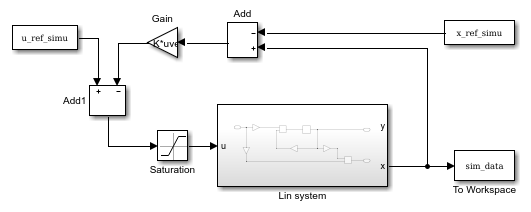
\includegraphics[width=\textwidth]{./LQR/not_generated/LQR_simulink.png}
	\caption{LQR in simulink}
	\label{fig:LQR simulink}
\end{figure}

\begin{figure}[H]
	\centering
	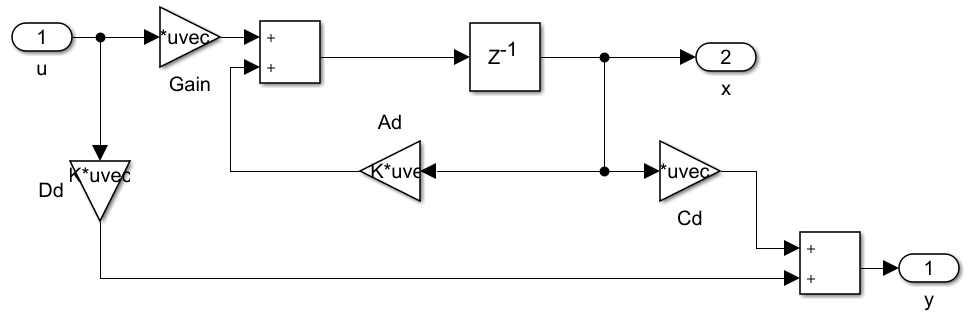
\includegraphics[width=0.6\textwidth]{./LQR/not_generated/simulink_subsys.png}
	\caption{LQR in simulink}
	\label{fig:LQR simulink subsystem}
\end{figure}

\subsection{Numerical values gain matrices LQR1 and LQR2}
The assignment specifically asked for the numerical values of the gains:

$$
K_{LQR_1} = 
\begin{bmatrix}
88.37 & 0 & 0 & 135.87 & 0 & 0 \\
0 & 88.37 & 0 & 0 & 135.87 & 0 \\
0 & 0 & 11.01 & 0 & 0 & 12.68 \\
\end{bmatrix}
$$

$$
K_{LQR_2} = 
\begin{bmatrix}
90.82 & 0 & 0 & 110.19 & 0 & 0 \\
0 & 90.82 & 0 & 0 & 110.2 & 0 \\
0 & 0 & 46.26 & 0 & 0 & 12.90 \\
\end{bmatrix}
$$

\subsection{Simulation results LQR1 and LQR2}

The assignment states the matrix $R=10^{-4} I_{3x3}$ for $LQR_1$ and $LQR_2$ , $Q=I_{6x6}$ for $LQR_1$ and $Q=diag(1,1,1,0,0,0)$ for $LQR_2$.

\begin{equation}
	J=x^TQx + u^TRu
\end{equation}

The trajectories followed by $LQR_1$ are about the same as $LQR_2$ this is visible on  figure~\ref{fig:simulink simulations LQR1 and LQR2 - trajects}. The inputs are also about the same this is visible on figure~\ref{fig:simulink simulations LQR1 and LQR2 - inputs}. This is not surprising at all as the keeper was already taking very smooth corners, reducing the weights on the speed $v_X$, $v_y$ and $v_{\omega}$ will reduce over-steering. 

%Except for the very severe over steering at the sharpest corner, there is nearly no over steering in this case. The very bad over steering is due to clipping on the inputs, figure~\ref{fig:least square opti simulation, better condition} very clearly has an to large input at the start and near the end of the trajectory. There is little difference between the two controllers. 

Figure~\ref{fig:trajectory LQR1 and LQR2 on 1 graph} contains both trajectory's on one graph, the bottom part of the picture is zoomed in on the corner where there is a slight difference. Here its visible that LQR2 does not optimize optimize on speed which makes it over steer a bit more in that corner. 

Figure~\ref{fig:simulink simulations LQR1 and LQR2 - inputs} clearly shows inputs on $F_x$ and $F_y$ that are clipped as they are suddenly flat at the maximum value. This obviously is a problem and explains why the keeper is not following the reference near the end and the start of the path on figure~\ref{fig:simulink simulations LQR1 and LQR2 - trajects}. 

\begin{figure}[H]
	\centering
	\begin{subfigure}[b]{0.45\textwidth}
		\includegraphics[width=\textwidth]{./LQR/LQR1_traject.png}
		\caption{$LQR_1$ trajectory}
		\label{fig:LQR1 traject}
	\end{subfigure}
	\begin{subfigure}[b]{0.45\textwidth}
		\includegraphics[width=\textwidth]{./LQR/LQR2_traject.png}
		\caption{$LQR_2$ trajectory}
		\label{fig:LQR2 traject}
	\end{subfigure}
	\begin{subfigure}[b]{0.55\textwidth}
		\includegraphics[width=\textwidth]{./LQR/LQR_compare.png}
		\caption{trajectory LQR1 and LQR2 on 1 graph}
		\label{fig:trajectory LQR1 and LQR2 on 1 graph}
	\end{subfigure}
	\caption{simulations with the controller in Simulink with $u_{ref}$ and $x_{ref}$}
	\label{fig:simulink simulations LQR1 and LQR2 - trajects}
\end{figure}


\begin{figure}[H]
	\centering
	\begin{subfigure}[b]{0.45\textwidth}
		\includegraphics[width=\textwidth]{./LQR/LQR1_input.png}
		\caption{$LQR_1$ input}
		\label{fig:LQR1 input}
	\end{subfigure}
	\begin{subfigure}[b]{0.45\textwidth}
		\includegraphics[width=\textwidth]{./LQR/LQR2_input.png}
		\caption{$LQR_2$ input}
		\label{fig:LQR2 input}
	\end{subfigure}
	\caption{input data of the simulations with the controller in simulink with $u_{ref}$ and $x_{ref}$}
	\label{fig:simulink simulations LQR1 and LQR2 - inputs}
\end{figure}


%\begin{figure}[H]
%	\centering
%	\begin{subfigure}[b]{0.45\textwidth}
%		\includegraphics[width=\textwidth]{./LQR/LQRincreasedR_traject.png}
%		\caption{$LQR_3$ traject}
%		\label{fig:LQR3 traject}
%	\end{subfigure}
%	\begin{subfigure}[b]{0.45\textwidth}
%		\includegraphics[width=\textwidth]{./LQR/LQRincreasedR_input.png}
%		\caption{$LQR_3$ input}
%		\label{fig:LQR3 input}
%	\end{subfigure}
%	\caption{input data of the simulations with the controller in simulink with $u_{ref}$ and $x_{ref}$ Q is increased to $10^{-1}$}
%	\label{fig:simulink simulations LQR1 and LQR2 - increased Q}
%\end{figure}

\subsection{The total simulation cost for each controller}
The LQR controller tries to minimize the  objective function $J = x^TQx + u^TRu$. Table~\ref{tab:total-simulation cost LQR} contains the actual values of the objective function. $LQR_2$ did not follow the reference path as close at $LQR_1$ and has an objective function that is about 0.01\% higher. The figures already showed that the difference was insignificant. Obviously its very hard to make any kind of concussions solely based on these figures.

\begin{minipage}{\linewidth}
	\centering
	\captionof{table}{total-simulation cost $LQR_1$, $LQR_2$} 
	\label{tab:total-simulation cost LQR} 
	\begin{tiny}\begin{tabular}{|c|c|}
\hline
\textbf{$LQR_1$}&\textbf{$LQR_2$}\\\hline
3.7231e+04&3.7236e+04\\\hline
\end{tabular}
\end{tiny}
\end{minipage}

\section{MPC controller}
\subsection{Formulate the MPC controller}
The MPC controller van be formally formulated as equation~\ref{eq:MPC def} or equation~\ref{eq:MPC maxtrix def}

\begin{equation}
	\begin{aligned}
		& \min_{x_N,u_N}
		& & \sum^{N}_{i=1} 	(x(k+i) - x_{ref}(k+i))^TQ(x(k+i) - x_{ref}(k+i)) \\
		& & & + \sum^{N-1}_{i=0} 	(u(k+i) - u_{ref}(k+i))^TR(u(k+i) - u_{ref}(k+i))\\
		& \text{subject to}
		& & x(k+1+i) = Ax(k+i) +Bu(k+i) \qquad    i=0,1,..., N-1\\
		&&& |u(k+i)| \leq u_{max} \qquad    i=0,1,..., N-1
	\end{aligned}
	\label{eq:MPC def}
\end{equation}

Or in matrix form:

\begin{equation}
	\begin{aligned}
		& \min_{\tilde{x}}
		& & \frac{1}{2} \tilde{x}^TH\tilde{x}+f^T\tilde{x} \\
		& \text{subject to}
		& & A_e \tilde{x} = b_e \\
		& & & A_i \tilde{x} \leq b_i
	\end{aligned}
	\label{eq:MPC maxtrix def}
\end{equation}

The Q and R are given in the assignment as: 
$$
R =
\begin{bmatrix}
10^{-4} & 0 & 0 \\
0 & 10^{-4} & 0 \\
0 & 0 & 10^{-4}
\end{bmatrix}
$$

$$
Q =
\begin{bmatrix}
10^{-4} & 0 & 0 & 0 & 0 & 0\\
0 & 10^{-4} & 0 & 0 & 0 & 0\\
0 & 0 & 10^{-4} & 0 & 0 & 0\\
0 & 0 & 0 & 0 & 0 & 0 \\
0 & 0 & 0 & 0 & 0 & 0 \\
0 & 0 & 0 & 0 & 0 & 0 
\end{bmatrix}
$$

\subsection{Remark on simulating MPC with Matlab}
One of the problems that occurs when simulating MPC with Matlab is that at the end of the simulation there are not enough steps left to do a full horizon. In this report the last optimal values calculated with a full horizon are used to simulate further to the end. The means that the last N-1 steps are not optimized individually. Thats also why all the simulation contain all the steps. (its easier to compare, especially because there is an sharp corner at the end and a large horizon will stop to soon otherwise)

\subsection{Simulation results}
Its clear from figure~\ref{fig:MPC simulation} that the larger the horizon the better the results.
\begin{figure}[H]
	\centering
	\begin{subfigure}[b]{0.45\textwidth}
		\includegraphics[width=\textwidth]{MPC/MPC_0_5_N_traj_input.png}
		\caption{horizon=N/2}
	\end{subfigure}
	\begin{subfigure}[b]{0.45\textwidth}
		\includegraphics[width=\textwidth]{MPC/MPC_2_N_traj_input.png}
		\caption{horizon=2N}
	\end{subfigure}
	\begin{subfigure}[b]{0.45\textwidth}
		\includegraphics[width=\textwidth]{MPC/MPC_N_traj_input.png}
		\caption{horizon=N}
	\end{subfigure}
	\caption{simulation of the MPC controllers, with different horizon sizes}
	\label{fig:MPC simulation}
\end{figure}

\subsection{Comparison MPC with LQR}
Figure~\ref{fig:compare LQR and MPC} contains the simulation results of the both the LQR and the MPC. The MPC is better then $LQR_2$ in all 3 cases. The MPC with a horizon of 2N is exceptionally good, while the other 2 smaller horizons are about the same.
\begin{figure}[H]
	\centering
	\includegraphics[width=0.5\textwidth]{MPC/compare.png}
	\caption{comparison $LQR_2$ and MPC methods}
	\label{fig:compare LQR and MPC}
\end{figure}

\subsection{Total-simulation cost}
Table~\ref{tab:total-simulation cost MPC} contains the actually values of the objective function. The relative difference is expressed as $\frac{J_{current}-J_{previous}}{J_{current}}$. The value of J goes about 10 times faster down from a horizon of N to 2N then from N/2 to N. Its also obvious that all 3 MPC situations are lower then $3.72 \cdot 10^{4}$, this again confirms that the MPC preforms better then the LQR algorithm.

\begin{minipage}{\linewidth}
	\centering
	\captionof{table}{total-simulation cost MPC with different horizons} 
	\label{tab:total-simulation cost MPC} 
	\begin{tiny}\begin{tabular}{|l|c|c|c|}
\hline
\textbf{horizon}&6.00e+00&1.20e+01&2.40e+01\\\hline
\textbf{J}&3.71e+04&3.71e+04&3.67e+04\\\hline
\textbf{relative difference previous value of J}&0.00e+00&-1.23e-03&-9.95e-03\\\hline
\end{tabular}
\end{tiny}
\end{minipage}
%J_N/J_0_5_N=0.9926
%J_2_N/J_N=0.9886

\subsection{Complexity}
The computational complexity of quadprog is hard to estimate as its not a method to solve quadratic problems. But rather a function that will decide for itself what underlying method it will use to solve the quadratic problem. The easiest way to get an idea of the complexity is to do some runs with different value for the horizon.

One has to be very careful when making conclusions from these results as the complexity will change if quadprog  changes the method it uses to solve the quadratic problem. As the complexity can suddenly change for some ranges of N. Table~\ref{tab:timings MPC} contains the run times for quadprog for different values of N. Its very clear that the complexity is of order 1, when N is twice as large the problem takes twice as much time.

\begin{minipage}{\linewidth}
	\centering
	\captionof{table}{average time quadprog for each iteration of the MPC with different horizons} \label{tab:timings MPC} 
	\begin{tiny}\begin{tabular}{|l|c|c|c|c|}
\hline
\textbf{horizon}&6.00e+00&1.20e+01&2.40e+01&5.00e+01\\\hline
\textbf{t(s)}&1.76e-02&3.21e-02&3.97e-01&1.82e-01\\\hline
\end{tabular}
\end{tiny}
\end{minipage}

The implication of this on the controller is that a bigger horizon can give better results but the optimization problem will take longer to solve. Here there is some kind of trade off between a fast small horizon controller and large horizon but slow controller.

The trade off should be made taking in account the speed of the process the controller is controlling. There is no point in putting a very fast controller on a slow process or vice versa. "If it takes 3 days to calculate the weather forecast of the next day, its pretty useless in practice."
\section{MPC controller with state constraint}
	\subsection{definition}
	The previous definition of the MPC controller(equation~\ref{eq:MPC def}) can be adjusted to incorporate the goalkeeper area (equation~\ref{eq:MPC def state const}). As the y borders are not symmetric the absolute value cannot be used as with y, only with x.
	
	\begin{equation}
		\begin{aligned}
			& \min_{x_N,u_N}
			& & \sum^{N}_{i=1} 	(x(k+i) - x_{ref}(k+i))^TQ(x(k+i) - x_{ref}(k+i)) \\
			& & & + \sum^{N-1}_{i=0} 	(u(k+i) - u_{ref}(k+i))^TR(u(k+i) - u_{ref}(k+i))\\
			& \text{subject to}
			& & x(k+1+i) = Ax(k+i) +Bu(k+i) \qquad    i=0,1,..., N-1\\
			&&& |u(k+i)| \leq u_{max} \qquad    i=0,1,..., N-1 \\
			&&& y_{min} \leq y(k+i)| \leq y_{max} \qquad    i=1,..., N \\
			&&& |x(k+i)| \leq x_{max} \qquad    i=1,..., N
		\end{aligned}
		\label{eq:MPC def state const}
	\end{equation}
	
	Figure~\ref{fig:MPC state constraint} contains the numerical results of the simulation of the MPC with state constraints. Even without increasing the $F_{max}$ the controller succeeds in taking a turn right before the $y_{max}$ border. 

\subsection{Simulation}
	The goalkeeper can't keep following the trajectory when it goes outside the goalkeeper area. The bigger the horizon the better the goalkeeper can adjust and make the corner more natural. A horizon of N/2 is clearly less elegant then a horizon of 2N. 
	\begin{figure}[H]
		\centering
		\begin{subfigure}[b]{0.45\textwidth}
			\includegraphics[width=\textwidth]{MPC_state_constraint/MPC_0_5_N_traj_input.png}
			\caption{MPC with horizon N/2}
		\end{subfigure}
		\begin{subfigure}[b]{0.45\textwidth}
			\includegraphics[width=\textwidth]{MPC_state_constraint/MPC_N_traj_input.png}
			\caption{MPC with horizon N}
		\end{subfigure}
		\begin{subfigure}[b]{0.45\textwidth}
			\includegraphics[width=\textwidth]{MPC_state_constraint/MPC_2_N_traj_input.png}
			\caption{MPC with horizon 2N}
		\end{subfigure}
		\caption{Simuation of MPC with state constrain forfor different horizons and fixed $F_{max}$ to the normal value}
		\label{fig:MPC state constraint}
	\end{figure}
	Figure~\ref{fig:MPC with state constrain, traject} illustrates the importance of the horizon even further. The right image is zoomed in on the border of the state constraint. The horizon of 0.5N clearly trouble adjusting too the state constraint.
	\begin{figure}[H]
		\centering
		\begin{subfigure}[b]{0.45\textwidth}
			\includegraphics[width=\textwidth]{MPC_state_constraint/compare.png}
			\caption{}
		\end{subfigure}
		\begin{subfigure}[b]{0.45\textwidth}
			\includegraphics[width=\textwidth]{MPC_state_constraint/compare_zoom.png}
			\caption{}
		\end{subfigure}
		\caption{Trajectory of MPC with state constrain for different horizons and fixed $F_{max}$ to the normal value}
		\label{fig:MPC with state constrain, traject}
	\end{figure}

\subsection{In-feasibilities}
	If the horizon is decreased to 5 the controller gets into trouble as can be observed in figure~\ref{fig:MPC state constraints N=5}. The quadratic optimization problem becomes infeasible and the simulation stops. If $F_{max}$  is increased by a factor of 10 then the controller does succeed in taking its turn. 
	
	\begin{figure}[H]
		\centering
		\begin{subfigure}[b]{0.45\textwidth}
			\includegraphics[width=\textwidth]{MPC_state_constraint/inf_traj_input.png}
			\caption{MPC with state constraint horizon=5}
			\label{fig:MPC state constraints N=5}
		\end{subfigure}
		\begin{subfigure}[b]{0.45\textwidth}
			\includegraphics[width=\textwidth]{MPC_state_constraint/inf_F10_traj_input.png}
			\caption{MPC with state constraint horizon=5 and $F_{max}=10 F_{max}$}
			\label{fig:MPC state constraints N=5 F=10F}
		\end{subfigure}
		\caption{MPC with state constrains and very low horizon value}
	\end{figure}
	
\subsection{Total-simulation cost}
	The total-simulation cost of the MPC with state constraint is clearly lower then that of the MPC without state constraint. This due to the fact that the state constrains keep the state value closer to the origin which obviously lowers the value of $J=x^TQx+u^TRu$.
	
	\begin{minipage}{\linewidth}
		\centering
		\captionof{table}{total-simulation cost MPC with state constraints for different horizons} 
		\label{tab:total-simulation cost MPC with state constrains} 
		\begin{tiny}\begin{tabular}{|l|c|c|c|}
\hline
\textbf{horizon}&6.00e+00&1.20e+01&2.40e+01\\\hline
\textbf{J}&3.36e+04&3.33e+04&3.29e+04\\\hline
\textbf{relative difference previous value of J}&0.00e+00&-7.45e-03&-1.16e-02\\\hline
\end{tabular}
\end{tiny}
	\end{minipage}

\subsection{Remark}
	Simulations with a horizon of N,$\frac{1}{2}$N or 2N give all most the same results with or without $F_{max}$ or $F_{max}$. The results of simulations with an increased $F_{max}$ can be seen in figure~\ref{fig:MPC with state constraints increased F} and figure~\ref{fig:MPC with state constraints increased F, traject comparison} in the appendix.
\section{MPC controller with terminal cost}
The previous cost function can be adjusted to incorporate the infinite horizon(equation~\ref{eq:MPC def terminal cost}) as was done with the lqr. This extra term will represent all the future values and hopefully reduce the dependence of the algorithm on the size of the horizon. This reduced dependence on the horizon length is visible in figure~\ref{fig:comparison MPC with terminal cost for different horizons}. 

Without the terminal cost the improvement going from a horizon of N to 2N is quiet drastic compared to the improvement from N/2 to N. But with the terminal cost the improvement going from N to N/2 and 2N to N is about the same. Figure~\ref{fig:MPC with and without terminal cost and different horizons} in the appendix also shows this. The dotted parallel lines vs the normal lines. This effect is also visible in Table~\ref{tab:total-simulation cost MPC with terminal cost} where the relative difference is not of order 2 going from a horizon of N to 2N compared to going from 0.5N to N. Where as this was of a factor 10 larger in case of the classical MPC.

\begin{equation}
	\begin{aligned}
		& \min_{x_N,u_N}
		& & \sum^{N-1}_{i=1} 	(x(k+i) - x_{ref}(k+i))^TQ(x(k+i) - x_{ref}(k+i)) \\
		& & & + \sum^{N-1}_{i=0} 	(u(k+i) - u_{ref}(k+i))^TR(u(k+i) - u_{ref}(k+i))\\
		& & & + (u(k+N) - u_{ref}(k+N))^TR(u(k+N) - u_{ref}(k+N))\\
		& \text{subject to}
		& & x(k+1+i) = Ax(k+i) +Bu(k+i) \qquad    i=0,1,..., N-1\\
		&&& |u(k+i)| \leq u_{max} \qquad    i=0,1,..., N-1
	\end{aligned}
	\label{eq:MPC def terminal cost}
\end{equation}

\begin{figure}[H]
	\centering
	\begin{subfigure}[b]{0.45\textwidth}
		\includegraphics[width=\textwidth]{MPC_term_cost/compare_ROI.png}
		\caption{with terminal cost}
	\end{subfigure}
	\begin{subfigure}[b]{0.45\textwidth}
		\includegraphics[width=\textwidth]{MPC/compare_horizon.png}
		\caption{without terminal cost}
	\end{subfigure}
	\caption{comparison MPC with terminal cost for different horizons}
	\label{fig:comparison MPC with terminal cost for different horizons}
\end{figure} 

\subsection{Comparison with and without terminal cost}
As mentioned earlier if the horizon is increased the computational cost per iteration is increased. The trajectory used in this assignment has a sharp corner near the end. Only a horizon of 2N was enough to take this corner properly.

\begin{figure}[H]
	\centering
	\begin{subfigure}[b]{0.45\textwidth}
		\includegraphics[width=\textwidth]{MPC_term_cost/compare_ROI_0_5_N.png}
		\caption{horizon=N/2}
	\end{subfigure}
	\begin{subfigure}[b]{0.45\textwidth}
		\includegraphics[width=\textwidth]{MPC_term_cost/compare_ROI_N.png}
		\caption{horizon=N}
	\end{subfigure}
	\begin{subfigure}[b]{0.45\textwidth}
		\includegraphics[width=\textwidth]{MPC_term_cost/compare_ROI_2_N.png}
		\caption{horizon=2N}
	\end{subfigure}
	\caption{comparison MPC with and without terminal cost, zoomed in on last corner}
\end{figure}

\subsection{Total-simulation cost}
As mentioned in the beginning of this section , the influence of the horizon is reduced because of the terminal cost term. This can also be observed in table~\ref{tab:total-simulation cost MPC with terminal cost}, the two relative differences do not increase by a factor of 10. 

\begin{minipage}{\linewidth}
	\centering
	\captionof{table}{total-simulation cost MPC with terminal cost for different horizons} 
	\label{tab:total-simulation cost MPC with terminal cost} 
	\begin{tiny}\begin{tabular}{|l|c|c|c|}
\hline
\textbf{horizon}&6.0000e+00&1.2000e+01&2.4000e+01\\\hline
\textbf{J}&3.6596e+04&3.6493e+04&3.6450e+04\\\hline
\textbf{relative difference previous value of J}&0.0000e+00&-2.8194e-03&-1.1722e-03\\\hline
\end{tabular}
\end{tiny}
\end{minipage}



\clearpage
\appendix
\section{Appendix: matlab code}
The following matlab files are important to run the code:
\begin{itemize}
	\item part4\_1\_lin\_approx.m
	\item part4\_2\_discrete\_matrix.m
	\item part4\_3.m
\end{itemize}

"part4\_1\_lin\_approx.m" contains code to set up the linear model. "part4\_2\_discrete\_matrix.m" contains the numerical analysis of the the discrete model. "part4\_3.m" contains the calculation of the matrices for 4 things:

\begin{itemize}
	\item the full state controller
	\item LQR with integral action
	\item full state controller with weight of 0.1
	\item The kallman filter
\end{itemize}

After the user executed a perticular section "part4\_3.m"  and so calculated the matrices its possible to run the following simulink files that use them:

\begin{itemize}
	\item part4\_3\_fullstate.slx
	\item part4\_3\_integrator.slx
	\item part4\_4\_simu\_LQG\_.slx
	\item part4\_4\_simu\_LQG\_kalmanF.slx
\end{itemize}


% \section*{Codes}
% \addcontentsline{toc}{section}{Codes}


\end{document}
